%=======================02-713 LaTeX template, following the 15-210 template==================
%
% You don't need to use LaTeX or this template, but you must turn your homework in as
% a typeset PDF somehow.
%
% How to use:
%    1. Update your information in section "A" below
%    2. Write your answers in section "B" below. Precede answers for all 
%       parts of a question with the command "\question{n}{desc}" where n is
%       the question number and "desc" is a short, one-line description of 
%       the problem. There is no need to restate the problem.
%    3. If a question has multiple parts, precede the answer to part x with the
%       command "\part{x}".
%    4. If a problem asks you to design an algorithm, use the commands
%       \algorithm, \correctness, \runtime to precede your discussion of the 
%       description of the algorithm, its correctness, and its running time, respectively.
%    5. You can include graphics by using the command \includegraphics{FILENAME}
%
\documentclass[11pt]{article}
\usepackage{amsmath,amssymb,amsthm}
\usepackage{graphicx}
\usepackage[margin=1in]{geometry}
\usepackage{fancyhdr}
\usepackage{listings}
\usepackage{float} 
\usepackage{subfig}

\setlength{\parindent}{0pt}
\setlength{\parskip}{5pt plus 1pt}
\setlength{\headheight}{13.6pt}
\newcommand\question[2]{\vspace{.25in}\hrule\textbf{#1: #2}\vspace{.5em}\hrule\vspace{.10in}}
\renewcommand\part[1]{\vspace{.10in}\textbf{(#1)}}
\newcommand\algorithm{\vspace{.10in}\textbf{Algorithm: }}
\newcommand\correctness{\vspace{.10in}\textbf{Output: }}
\newcommand\runtime{\vspace{.10in}\textbf{Running time: }}
\pagestyle{fancyplain}
\lhead{\textbf{\NAME\ (\ANDREWID)}}
\chead{\textbf{Project\HWNUM}}
\rhead{\today}
\begin{document}\raggedright
%Section A==============Change the values below to match your information==================
\newcommand\NAME{Yao Xiao}  % your name
\newcommand\ANDREWID{2019180015}     % your andrew id
\newcommand\HWNUM{4}              % the homework number
%Section B==============Put your answers to the questions below here=======================

% no need to restate the problem --- the graders know which problem is which,
% but replacing "The First Problem" with a short phrase will help you remember
% which problem this is when you read over your homeworks to study.

WebAuthn uses public key certificates instead of passwords to complete user registration and identity authentication (login). 
It is more like an enhancement or supplement to existing identity authentication. 
In order to ensure the security of communication data, it is generally based on HTTPS (TLS) communication.

\begin{enumerate}
    \item Server: It can be considered as a relying party (Relying Party), it will store the user's public key and is responsible for user registration, authentication.
    \item Browser: Credential Management API with WebAuthn is required
    \item Authentication module (Authenticator): It can create, store, and retrieve identity credentials. 
    It is generally a hardware device (smart • card, USB), or it may have been integrated into your operating system (such as Windows Hello).
\end{enumerate}

\question{1}{Register} 


\part{a} \textbf{Initiate a registration request}

\part{b} \textbf{The server returns Challenge, user information, relying party information}

\part{c} \textbf{The browser calls the authentication module to generate a certificate}

This is an asynchronous task, and the JS script calls the browser's navigator.credentials.create to create a certificate.

\begin{lstlisting}
getMakeCredentialsChallenge({username, name})
        .then((response) => {
            let publicKey = preformatMakeCredReq(response);
            return navigator.credentials.create({ publicKey })
        })
        .then((response) => {
            console.log(response);
            let makeCredResponse = publicKeyCredentialToJSON(response);
            return sendWebAuthnResponse(makeCredResponse)
        })
        .then((response) => {
            if(response.status === 'ok') {
                loadMainContainer()   
            } else {
                alert(`Server responed with error. The message is: ${response.message}`);
            }
        })

\end{lstlisting}

\part{d} \textbf{The authentication module creates a pair of public / private key and attestation data}

\part{e} \textbf{The authentication module sends the public key / Credential rawID / attestation to the browser}

\part{f} \textbf{The browser sends Credential to the server}

\part{g} \textbf{Server completes registration}



\question{2}{Authentication}

Same as most steps for registration

Call navigator.credentials.get of the browser to retrieve the certificate.

\begin{lstlisting}
getGetAssertionChallenge({username})
        .then((response) => {
            console.log(response)
            let publicKey = preformatGetAssertReq(response);
            return navigator.credentials.get({ publicKey })
        })
        .then((response) => {
            console.log(response)
            let getAssertionResponse = publicKeyCredentialToJSON(response);
            return sendWebAuthnResponse(getAssertionResponse)
        })
        .then((response) => {
            if(response.status === 'ok') {
                loadMainContainer()   
            } else {
                alert(`Server responed with error. The message is: ${response.message}`);
            }
        })

\end{lstlisting}

\question{3}{Task}

\part{a} \algorithm{}
\begin{lstlisting}
import urllib
import base64
import getpass
import urllib3
urllib3.disable_warnings(urllib3.exceptions.InsecureRequestWarning)
import base64

import simplejson
import requests
import cbor2 as cbor
from fido2.hid import CtapHidDevice
from fido2.client import Fido2Client



class Fido2HttpClient(object):
    session = None
    server = None
    dev = None
    ssl_verify = True
    begin_url = None
    complete_url = None
    is_authenticated = False
    verbose = False

    def authenticate_to(self,
            server, begin_endpoint, complete_endpoint,
            session=None, append_to_data=None, append_to_headers=None):
        self.server = server
        self.init_dev()
        begin_url = urllib.parse.urljoin(server, begin_endpoint)
        complete_url = urllib.parse.urljoin(server, complete_endpoint)

        if self.dev:
            if session:
                self.session = session
            if not self.session:
                self.session = requests.session()

            self.begin(begin_url,
                append_to_headers=append_to_headers)
            self.complete(complete_url,
                append_to_data=append_to_data,
                append_to_headers=append_to_headers)
        return self.is_authenticated

    def log(self, *args):
        if self.verbose: print(args)

    def ask_for_interaction(self):
        print('Touch your authenticator device...')

    def no_device_found(self):
        print('No FIDO device found')

    def authenticated(self):
        print('Authenticated')

    def say_not_authenticated(self, data):
        print('Not Authenticated')

    def init_dev(self):
        self.dev = next(CtapHidDevice.list_devices(), None)
        if not self.dev:
            self.no_device_found()            

    def begin(self, begin_url, append_to_headers=None):
        headers = {}
        if append_to_headers:
            for k in append_to_headers:
                headers[k] = append_to_headers[k]

        r = self.session.post(begin_url,
            verify=self.ssl_verify,
            headers=headers)

        self.begin_data = cbor.loads(r.content)
        self.log('BEGIN RESPONSE: ', self.begin_data)

    def complete(self, complete_url, append_to_data=None, append_to_headers=None):
        fido2_client = Fido2Client(self.dev, self.server)

        pubkey = self.begin_data['publicKey']
        challenge = base64.b64encode(pubkey['challenge'])
        challenge = challenge.decode('utf-8')
        allow_list = [{
            'type': 'public-key',
            'id': pubkey['allowCredentials'][0]['id'],
        }]

        self.ask_for_interaction()
        try:
            assertions, client_data = fido2_client.get_assertion(
                pubkey['rpId'],
                challenge,
                allow_list)
        except ValueError:
            assertions, client_data = fido2_client.get_assertion(
                pubkey['rpId'],
                challenge,
                allow_list,
                pin=getpass.getpass('Please enter PIN:'))

        assertion = assertions[0]
        self.log('ASSERTION: ', assertion)
        self.log('CLIENT DATA: ', client_data)

        user_data = {}
        if append_to_data:
            user_data = append_to_data
        user_data = base64.b64encode(simplejson.dumps(user_data).encode('utf-8'))

        data = {
            'credentialId': assertion.credential['id'],
            'authenticatorData': assertion.auth_data,
            'clientDataJSON': client_data,
            'signature': assertion.signature,
            'user_data': user_data,
        }
        body = cbor.dumps(data)
        headers = {'content-type': 'application/cbor'}
        if append_to_headers:
            for k in append_to_headers:
                headers[k] = append_to_headers[k]

        r = self.session.post(complete_url,
            verify=self.ssl_verify,
            headers=headers,
            data=body
        )
        self._last_response = r

        data = cbor.loads(r.content)
        self.log('Response: ', data)
        if 'status' in data and data['status'] == 'OK':
            self.is_authenticated = True
        else:
            self.is_authenticated = False

        if self.is_authenticated: self.authenticated()
        else: self.say_not_authenticated(data)
        return self.is_authenticated

    def get_last_response(self):
        return self._last_response

\end{lstlisting}



\part{b} \correctness


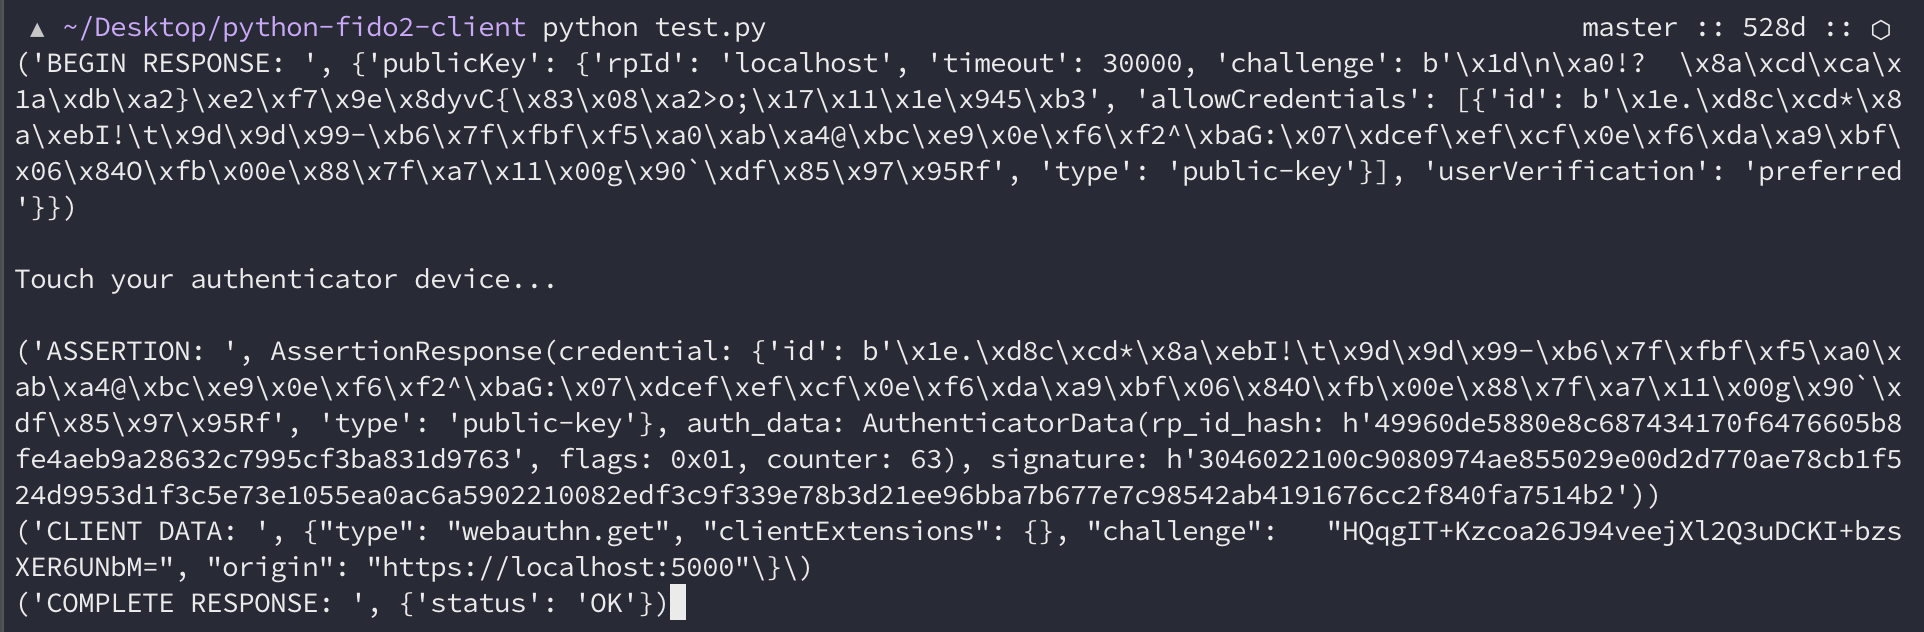
\includegraphics[width=0.85\textwidth]{Fig1}




\end{document}
